\subthesischapter{Arquitectura del software}
En la aplicación se usó como arquitectura de software el \hyperlink{page: abbidx}{MVC}, un patrón de software comúnmente utilizado para implementar datos (Modelo), interfaces de usuario (Vista) y lógica de control (Controlador), que enfatiza una separación entre la lógica de negocios y su visualización. En la Figura \ref{fig: software-architecture} se muestra el MVC correspondiente a la aplicación de juego serio.

\begin{figure}[ht]
    \centering
    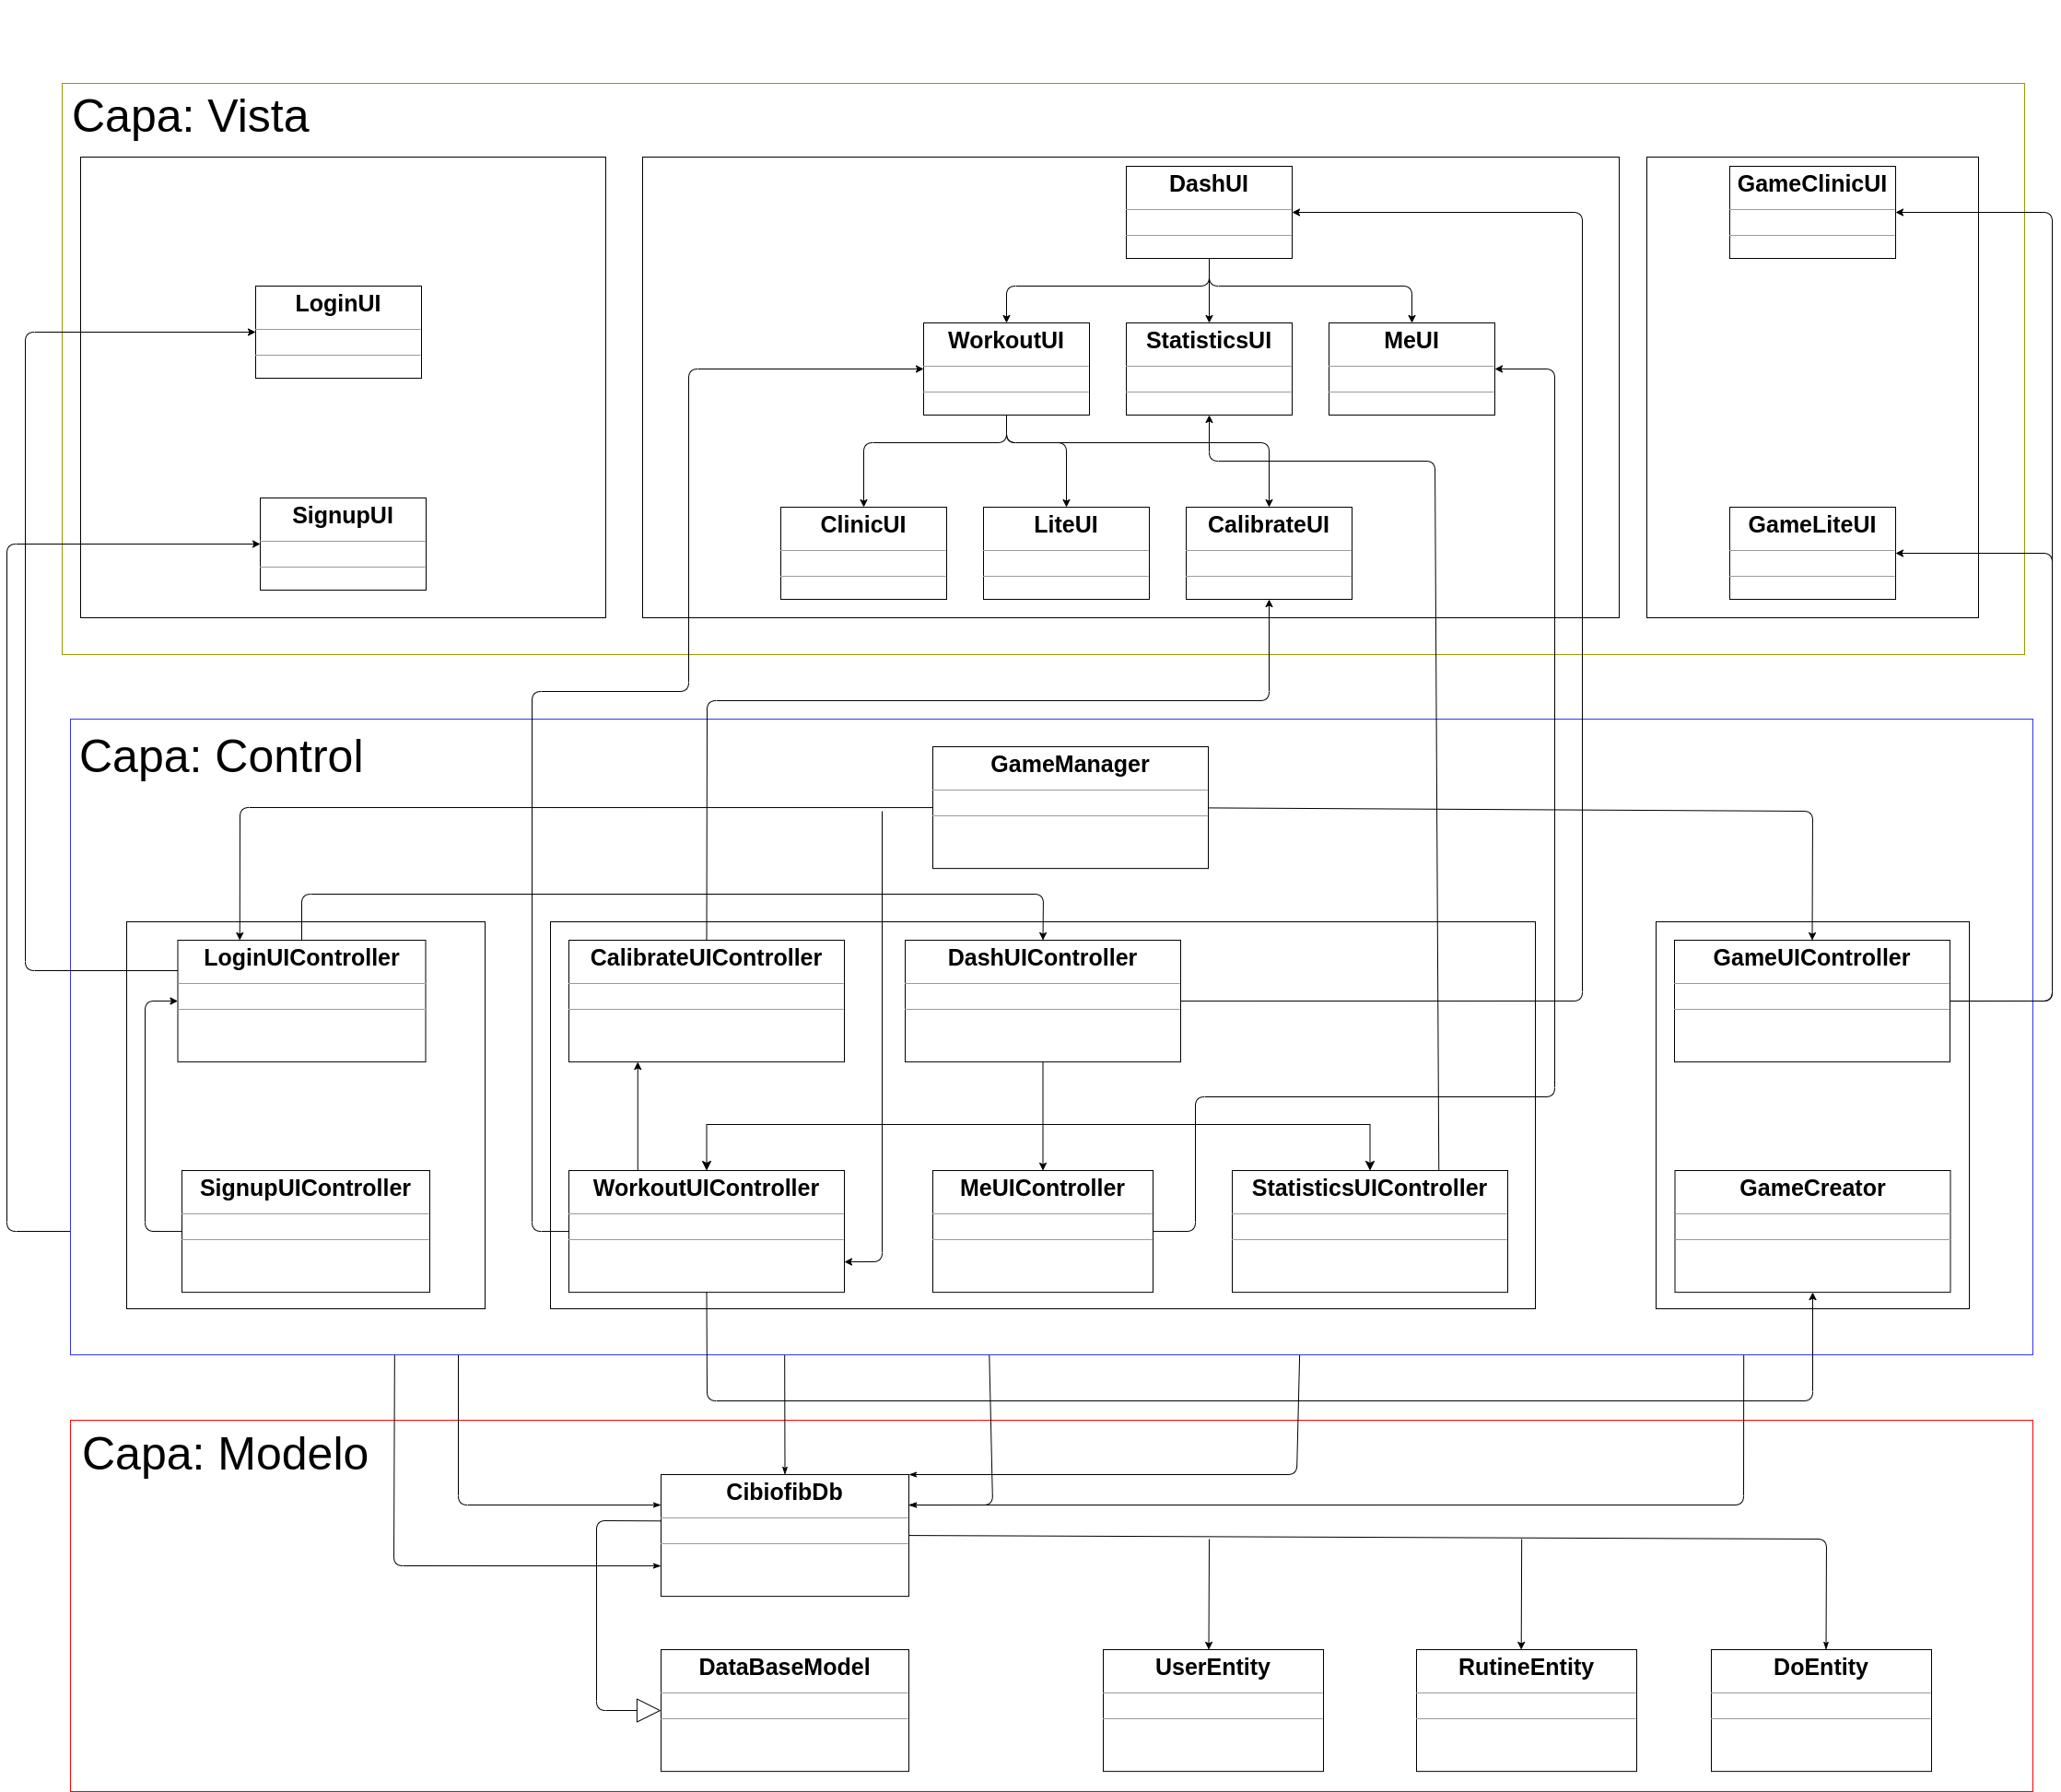
\includegraphics[scale=0.18]{images/software-architecture.png}
    \caption{Diagrama de clase de diseño}
    \label{fig: software-architecture}
\end{figure}



